%************************************************
\chapter{Introduction}\label{ch:introduction}
%************************************************

Satisfiability Modulo Theories (SMT) solvers are automated reasoning (AR) tools that have become essential in a wide range of formal reasoning tasks, including program verification, model checking, and interactive theorem proving.
Their efficiency and expressive power enable them to handle complex logical proofs and verifications with speed.
At the same time, the growing reliance on SMT solvers raises a fundamental question of trust: \textit{can we be confident that the results produced by these highly complex SMT solvers are correct?}

Despite their central role, SMT solvers are large software systems with complex architectures \cite{cvc5}, often comprising hundreds of thousands of lines of code.
This complexity makes it extremely difficult to guarantee their correctness.
The annual SMT-COMP competition \cite{smtcomp2015–2018,SMT-COMP}, regularly uncovers cases where different solvers disagree on the satisfiability status of the same benchmark.
Such discrepancies highlight the practical risk of relying blindly on solver outputs in safety critical applications.

A natural response to this problem is to attempt the certification of the solver itself.
However, formally verifying such a large and complex codebase is highly impractical.
Simplifying a solver’s design to ease certification would necessarily come at the expense of performance, which is a key factor in their adoption.
Moreover, certification tends to ``freeze'' the implementation: once a system is verified, the integration of new features, heuristics, or optimizations becomes prohibitively costly, since each change would require a new certification effort.
Consequently, directly certifying solvers might not scale with the pace of their development.

A first approach is to develop a certified solver in a proof assistant such as the IsaSAT solver \cite{fleury:tel-02963301,fleury:hal-01904647} that is a fully verified SAT solver developed in Isabelle/HOL \cite{isabelle-hol-ref}.
IsaSAT refines a formal specification of conflict-driven clause learning (CDCL) \cite{dpll} into executable code, and has been demonstrated to achieve competitive performance in SAT solving \cite{EDA-challenge}.
This approach offers strong guarantees about the correctness of the implementation itself, since the solver is extracted from a machine-checked formalization.
While IsaSAT has been extended to output DRAT proofs, these proofs are not yet checked within the verified framework, and therefore do not provide the same level of end-to-end certification as approaches that combine solver output with independently verified proof checking.
In this respect, IsaSAT advances the state of the art by providing a verified implementation of SAT solving, but it does not yet close the gap toward fully certifying solver results.
Moreover, the restriction to SAT limits its applicability in domains where SMT reasoning is required.


An alternative line of research is the \emph{proof logging} \cite{proof-logging} where the approach is to certify the \emph{results} rather than the solver implementation.
The proof logging is a technique for automatically reviewing the reasoning steps of a proof engine by a separate tool.
This is achieved by requiring the solver to produce a proof, or certificate, of its output.
An SMT proof formally records the logical reasoning that leads to a solution, enabling independent verification by a separate proof checker.
Crucially, the task of proof checking is conceptually simpler and typically much faster than solving itself.
This decouples the trust in solver results from the correctness of the solver’s implementation, thereby providing a more practical path toward trustworthy automated reasoning.
Several proof assistants employ \emph{hammers} for discharging goals to automatic theorem provers (ATPs), including SMT solvers.
Examples include Sledgehammer \cite{Sledgehammer} for Isabelle/HOL and CoqHammer \cite{coqhammer1,coqhammer2} for Coq.
The hammer translates the conjecture and facts supplied by the user or harvested from the context to the input language of the back-end, invokes it, and in the case of success attempts to reconstruct the proof in the logic of the proof assistant, based on a trace of the proof found by the back-end.


\begin{figure}[t]
    \centering
    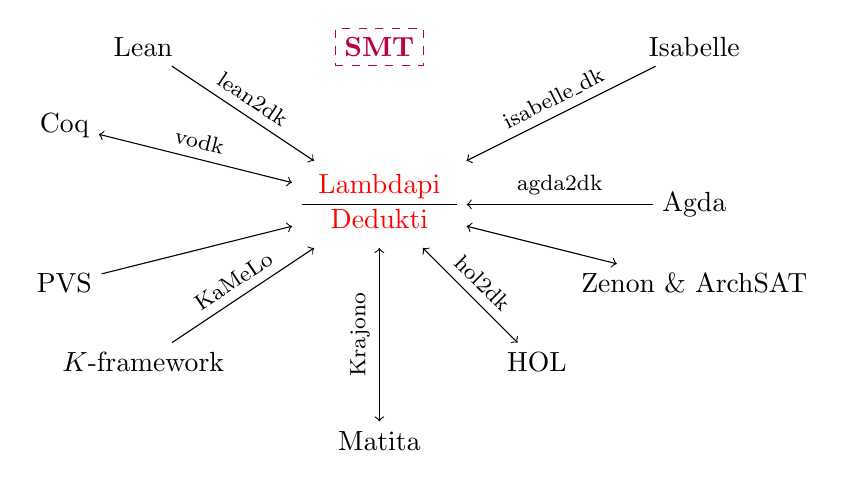
\begin{tikzpicture}
      \path (0,0) node (lp) {\begin{tabular}{c}
        \textcolor{red}{Lambdapi} \\
        \hline
        \textcolor{red}{Dedukti}
      \end{tabular}}
            (-4,1) node (coq) {Coq}
            (-3,2) node (lean) {Lean}
            (0,2) node [draw, dashed, purple] (smt) {\color{purple}\textbf{SMT}}
            (4,2) node (isa) {Isabelle}
            (4,0) node (agda) {Agda}
            (-3,-2) node (k) {$\mathbb{K}$-framework}
            (0,-3) node (mat) {Matita}
            (2,-2) node (hol) {HOL}
            (-4,-1) node (pvs) {PVS}
            (4,-1) node (ze) {Zenon \& ArchSAT}
            ;
      % \draw[->,red, thick] (smt) -- (lp) node[midway,sloped,above]
      % {\footnotesize{Carcara}};
      \draw[->] (lean) -- (lp) node[midway,sloped,above] {\footnotesize{lean2dk}};
      \draw[->] (isa) -- (lp) node[midway,sloped,above] {\footnotesize{isabelle\_dk}};
      \draw[->] (agda) -- (lp) node[midway,sloped,above] {\footnotesize{agda2dk}};
      \draw[<->] (ze) -- (lp) node[midway,sloped,above] {};
      \draw[<->] (hol) -- (lp) node[midway,sloped,above] {\footnotesize{hol2dk}};
      \draw[<->] (mat) -- (lp) node[midway,sloped,above] {\footnotesize{Krajono}};
      \draw[->] (pvs) -- (lp);
      \draw[->] (k) -- (lp) node[midway,sloped,above] {\footnotesize{KaMeLo}};
      \draw[<->] (coq) -- (lp)  node[midway,sloped,above] {\footnotesize{vodk}};
    \end{tikzpicture}
    \caption{Lambdapi, an assembly language for proof systems.}
    \label{fig:interop}
\end{figure}